\documentclass{article}
\usepackage[a4paper]{geometry}
\usepackage{graphicx}
\usepackage{hyperref}
\usepackage{float}
\usepackage{tikz}
\usepackage{amsmath}
\usepackage{amssymb}
\usepackage{graphicx}
\usepackage[affil-it]{authblk}\hypersetup{
    colorlinks,
    citecolor=black,
    filecolor=black,
    linkcolor=black,
    urlcolor=black
}
\usepackage{apacite}
\usepackage[authoryear]{natbib}

\setlength{\parindent}{0pt}
\setlength{\parskip}{1em}

\title{Evolutionary Models with a Large Number of Genes}
\author{
    Mher Saribekyan, Suren Hakobyan, Davit Badalyan\\
    Instructor: Varazdat Stepanyan 
}
\affil{American University of Armenia}
\date{December 2024}
\begin{document}
\maketitle
\newpage
\tableofcontents
\newpage

\section{Introduction}
Have you ever asked yourself how humanity has reached its current state of being? Have you ever wondered how some species (including humans) survived throughout centuries of changing environment, while others went extinct? The answer to these and many other questions lie in the broad study of evolution. 

According to Cambridge Dictionary, evolution is defined as \textit{"the way in which living things change and develop over millions of years."} Living things inevitably change over time due to multiple reasons. For example, a long-term food shortage caused by the change in the environment can force a given species to eat less, which over time will affect the next generations of the same species. The new generations might become more and more resistant to starvation and require less nutrition to survive. During this transition, many representatives of the species might die, and in some cases the species might fail to adapt and go extinct. However, if it \textbf{evolves} successfully, then the species will continue it's existence in the new environment, which might once again change in the future. 

A more scientific definition to the term evolution was given by Douglas Futuyma in his popular textbook.

\begin{quotation}
    [biological evolution] is change in the properties of groups of organisms over the course of generations…it embraces everything from slight changes in the proportions of different forms of a gene within a population to the alterations that led from the earliest organism to dinosaurs, bees, oaks, and humans.
\end{quotation}

Evolution can occur by different means, such as natural selection, genetic drift, mutation, migration and so on. This report will simulate the process of species evolving over time by adapting to their environment through mutations and natural selection. It will explore scenarios with different starting conditions, where diverse creatures with unique genes inhabit varying environments. The study will examine how these genes mutate over time and determine which mutations dominate in each specific setting.
\newpage

\section{Glossary}

Let one first establish some notions which are being discussed throughout this report. These definitions will help the reader more easily grasp the material of this paper, including terms related to biology and mathematics.

\subsection{Natural Selection}

Elena Racevska defined natural selection as follows.

\begin{quotation}
    Natural selection is a process by which organisms that are better adapted to specific pressures of their environment tend to survive longer and produce more offspring, thus ensuring the preservation and multiplication of those favorable traits through generations, at the expense of the less advantageous ones.
\end{quotation}

If there were no limitations on any species, then it would boundlessly grow. The nature is preventing this by imposing various limitations and creating an environment where species need to survive by adapting to the realities around them. Such limitations may include food limitations, disadvantageous climate conditions, diseases, natural disasters, rival species and so on. In this way, the nature "selects" those species which will be able to reproduce and hence create an evolutionary change. The article published at Stanford University makes in interesting analogy. 

\begin{quotation}
    Much like breeders choose which of their animals will reproduce and thereby create the various breeds of domesticated dogs, pigeons, and cattle, nature effectively “selects” which animals will breed and creates evolutionary change just as breeders do.
\end{quotation}

\subsection{Mutation}

A mutation is a change in a genetic sequence. In biology, it is usually discussed as a negative alteration of a creature's genetic code, which causes various genetic diseases. In the scope of this paper, a mutation is the change in the genome of an offspring compared to genome of it's parent. That is, when a creature reproduces, the genes of it's off-springs might be slightly modified (also called somatic mutation). Some traits of the offspring might remain the same, others might change.

\subsection{Asexual Reproduction}

The species which is being simulated in this report reproduce asexually. The Journal of Evolutionary Biology put the definition of asexual reproduction in the following manner.

\begin{quotation}
    Asexual reproduction occurs when an individual produces new individuals that are genetically identical to the ancestor at all loci in the genome, except at those sites that have experienced somatic mutations.
\end{quotation}

In simpler terms, each representative of a species reproduce on its own and copies itself, with a chance that the offspring (copy) will have a slightly mutated, modified genome.

\subsection{Manhattan Distance}

For any two points $p, q \in \mathbb{R}^n$, the manhattan distance (also called taxicab distance) is defined as

\[
    d_T(p, q) = \|p - q\|_T = \sum_{i = 1}^n |p_i - q_i| 
\]

In particular, for a plane ($\mathbb{R}^2$) the manhattan distance between two points is $d_2(p, q) = |p_1 - q_1| + |p_2 - q_2|$.

\newpage

\section{Simulation Setting}

Let one first define the simulation setting. Each simulation is a collection of time steps. First, the environment and all of its components are being initialized, then the generated entities iterate through a predefined number of steps, and finally at the end the data is being collected, analyzed and visualized.

\subsection{Creature}

A creature is a single representative of the species one is observing. Each time step, a creature is looking around in search for food, goes towards the food if it sees any, and eats the food if the food is nearby. The creature can also decide to battle another creature if they are in the same location and eat them in case of victory. If in a favorable position, the creature will reproduce, creating an offspring.

Each creature has a genome, a position in the environment and an energy level. Let one discuss each of these separately.

\subsubsection{Genome}

The genome of a creature is what defines the characteristics (traits) of that creature. It resembles the DNA of the creature which is predefined by nature. The genome and it's change through generations is how evolution is observed, and it is the primary focus of this study.

The genome consists of 5 individual genes, each of which depicts a certain trait. Here are the general descriptions of the traits. Note the possible values taken for each trait are only integers.

\begin{enumerate}
    \item \textbf{Speed} - determines the maximal distance that the creature can travel in a single time step. Takes values between 1 and 4.
    \item \textbf{Eyesight} - determines the area which is visible to the creature. It is mostly used to locate food and move towards it. Takes values between 0 and 7.
    \item \textbf{Aggression} - determines if the creature will engage in a fight or not. A higher aggression value means that the creature is more likely to start a battle, while a lower value means the creature is more likely to avoid contact and mind it's own business. Takes values between 0 and 7.
    \item \textbf{Strength} - determines the physical abilities of the creatures in case of a fight. A creature with a higher strength value is more likely to win the battle against a creature with a lower strength value. Takes values between 1 and 16.
    \item \textbf{Stamina} - determines the endurance of the creature, how long can the creature last without resources and at most how much energy it can store in itself. Takes values between -7 and 8.
\end{enumerate}

\subsubsection{Position}

The position of a creature describes the location of the creature in a given environment. Position has different meanings depending on different environments. For example, the position of a creature on a plane is a coordinate pair $(x, y)$, on a line its a single number, in space its a coordinate triple $(x, y, z)$ and so on. For each environment, the position will be separately defined, which majorly affects on how creatures move, hence affecting the evolution.

\subsubsection{Energy}

The energy of a creature showcases the physical power left in the creature to continue surviving. A non-positive value for the energy means that the creature has no power left and hence dies. Each time step, every creature loses energy on moving and supporting their physical existence (see section 3.1.5). Creatures gain energy by eating food or other creatures if they win in a battle. The energy is also used to reproduce, since a certain threshold of energy must be satisfied so that the creature is able to reproduce.

Each creature has maximal energy. It is showing the energy capacity of the creature, how much energy can the creature store in itself. The maximal energy is defined as

\[
    ME(\text{gene}) = 8 + \text{stamina}
\]

\subsubsection{Memory Optimization}

In order to make the simulation possible to run for relatively big populations in a reasonable time frame, the creatures were designed to take as less space as possible. In the current implementation, each creature is an unsigned 32-bit integer, where (starting from the left) the first 16 bits represent its genome, the next 12 bits represent its position and the last 4 bits represent its current energy. The figures below visualizes the structure of an individual creature more vividly.

\begin{figure}[!h]
\begin{center}
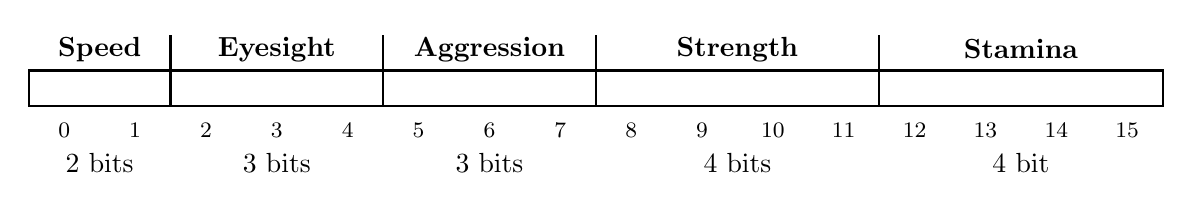
\begin{tikzpicture}[scale=0.9]
    % Draw the main rectangle for the 32 bits
    \draw[thick] (-0.5, 0) rectangle (15.5, 0.5);
    
    % Draw internal divisions for fields
    \foreach \x in {1.5, 4.5, 7.5, 11.5} {
        \draw[thick] (\x, 0) -- (\x, 1);
    }

    % Label the fields
    \node at (0.5, 0.8) {\textbf{Speed}};
    \node at (3, 0.8) {\textbf{Eyesight}};
    \node at (6, 0.8) {\textbf{Aggression}};
    \node at (9.5, 0.8) {\textbf{Strength}};
    \node at (13.5, 0.8) {\textbf{Stamina}};
    
    % Add labels for the bit positions (0-31)
    \foreach \x in {0, 1, ..., 15} {
        \node[anchor=north] at (\x, -0.1) {\footnotesize \x};
    }

    % Field descriptions under each field
    \node at (0.5, -0.8) {2 bits};
    \node at (3, -0.8) {3 bits};
    \node at (6, -0.8) {3 bits};
    \node at (9.5, -0.8) {4 bits};
    \node at (13.5, -0.8) {4 bit};
\end{tikzpicture}
\caption{Gene storage}
\end{center}
\end{figure}
\begin{figure}[!h]
\begin{center}
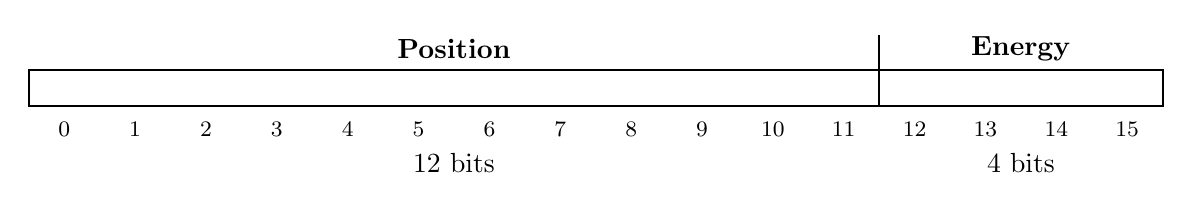
\begin{tikzpicture}[scale=0.9]
    % Draw the main rectangle for the 32 bits
    \draw[thick] (-0.5, 0) rectangle (15.5, 0.5);
    
    % Label the fields
    \node at (5.5, 0.8) {\textbf{Position}};
    \draw[thick] (11.5, 0) -- (11.5, 1);
    \node at (13.5, 0.8) {\textbf{Energy}};
    
    % Add labels for the bit positions (0-31)
    \foreach \x in {0, 1, ..., 15} {
        \node[anchor=north] at (\x, -0.1) {\footnotesize \x};
    }

    % Field descriptions under each field
    \node at (5.5, -0.8) {12 bits};
    \node at (13.5, -0.8) {4 bits};
\end{tikzpicture}
\caption{Position storage}
\end{center}
\end{figure}

\newpage This makes a huge impact on memory usage. Let one compare this approach with the one where each trait, position and energy is stored in a separate 32 bit integer. If one has $n$ creatures at a given time step, then the implementation described above will require $32n$ bits for storing all the creatures. On the contrary, if one uses 32 bit numbers for each parameter of the creature, then it would require at least $224$ bits to store one creature and $224n$ bits for storing the whole population, 7 times more than with bit manipulations. For example, let $n = 100$, a number which was exceeded by the simulations many times, so it is not a very high number to consider. With bit manipulations, the total memory required is 3200 bits, that is 400 bytes. Without bit manipulation one looks at 22400 bits, which is roughly 2.73 kilobytes.

\subsubsection{Energy Loss}

The energy loss is a function which determines how much energy does the creature lose in order to support itself. For the purposes of this paper, the energy loss function has been chosen to be the following.

\[
EL(\text{gene}) = \left[ 0.35 \left(
\text{steps} 
+ \left\lceil \frac{\text{eyesight}}{3} \right\rceil 
+ \left\lfloor \frac{\text{aggression}}{5} \right\rfloor 
+ \left\lfloor \sqrt{\text{strength}} \right\rfloor 
+ \left\lfloor \frac{\text{stamina}}{7} + 1 \right\rfloor
\right) \right]
\]
\[0 \leq \text{steps} \leq \text{speed}\in\{1,2,3,4\}\]
\[\text{eyesight}\in\{0,1,...,7\}\]
\[\text{aggression}\in\{0,1,...,7\}\]
\[\text{strength}\in\{1,2,...,16\}\]
\[\text{stamina}\in\{-7,-6,...,8\}\]

The steps in the energy loss function is the number of steps taken in the given move. For example, the creature might have speed with value 4 but only do 2 steps to reach the food nearby, so it only spends 2 units of energy, but not 4. Other traits makes the creature constantly use energy to support them.

It is important to understand that the energy loss function is specific to the purpose of the simulation. Depending on what simulation one is doing and what the environment is, this function can have a completely different form. This function is good enough for the purposes of this paper. The differences in constants tries to showcase how some traits are "cheaper" to maintain, while others require more energy. However, it is to be noted here that if some trait is easier to maintain that doesn't mean that creatures are going to always favor it in any environment, the simulations and results are much more complex than that.

\subsection{Food}

As already discussed above, one of the means for creature to gain energy and support their further survival is through finding and consuming food. Food is a naturally generating unit. After each time step, food is being updated based on the food cap set at the beginning of the simulation. Usually, it is set to meet a certain percentage of available area. During every time step the missing food is naturally replenished to keep the environment as constant as possible.

\subsection{Reproduction and Mutations}

The species in question reproduce asexually. If a creature's energy level increases more than $80\%$ of its maximal possible energy, it reproduces, gives 1 offspring, and loses $50\%$ of it's current energy because of it. Reproduction is the only way a creature can spawn in naturally in the simulation. The only exceptions are the initially generated creatures at the beginning of the simulation.

Each individual trait of the gene has an $8\%$ chance of mutating and increasing/decreasing its value by 1 unit. If one denotes $M$ as the event of getting mutations, then the probability of getting at least one mutation happening in an offspring is

\[
    \mathbb{P}(M \geq 1) = 1 - \mathbb{P}(M = 0) = 1 - 0.92^5 \approx 0.341 
\]

One can argue that this percentage is quite high and would have a point. However, each additional step in a simulation exponentially adds the waiting time for that simulation, hence the mutation percent is high so that meaningful results can be obtained in a reasonable amount of time.

\newpage

\section{Results}

\subsection{Grid Environment}

The grid environment is a plane where the values on each axis are integers. The position of the creatures is expressed by two coordinates: $x$ and $y$. Since there are 12 bits to store the position of the creature, the first 6 bits will store $x$ and the other 6 will store the value of $y$. This means that $0 \leq x, y \leq 63$, since one can have 64 values with 6 bits for each coordinate. That also fixes the size of the grid: 64 x 64, 64 possible values for each coordinate.

\subsubsection{Scenario 1: Average Gene}

In this scenario, the starting gene for all creatures is set to be a gene with average traits. More specifically, the gene is represented by the following 16 bits: 0101101110001000, which means 2 speed, 3 eyesight, 3 aggression, 8 strength and 1 stamina.

\textbf{Simulation 1} - 1\% Food, 1\% Creatures

\textbf{Simulation 2} - 1\% Food, 5\% Creatures

\textbf{Simulation 3} - 1\% Food, 20\% Creatures

\textbf{Simulation 4} - 5\% Food, 1\% Creatures

\textbf{Simulation 5} - 5\% Food, 5\% Creatures

\textbf{Simulation 6} - 5\% Food, 20\% Creatures

\textbf{Simulation 7} - 20\% Food, 1\% Creatures

\textbf{Simulation 8} - 20\% Food, 5\% Creatures

\textbf{Simulation 9} - 20\% Food, 20\% Creatures

\subsubsection{Scenario 2: Random}

In this scenario, every creature starts up with a random gene.

\textbf{Simulation 1} - 1\% Food, 1\% Creatures

\textbf{Simulation 2} - 1\% Food, 5\% Creatures

\textbf{Simulation 3} - 1\% Food, 20\% Creatures

\textbf{Simulation 4} - 5\% Food, 1\% Creatures

\textbf{Simulation 5} - 5\% Food, 5\% Creatures

\textbf{Simulation 6} - 5\% Food, 20\% Creatures

\textbf{Simulation 7} - 20\% Food, 1\% Creatures

\textbf{Simulation 8} - 20\% Food, 5\% Creatures

\textbf{Simulation 9} - 20\% Food, 20\% Creatures

\begin{center}
    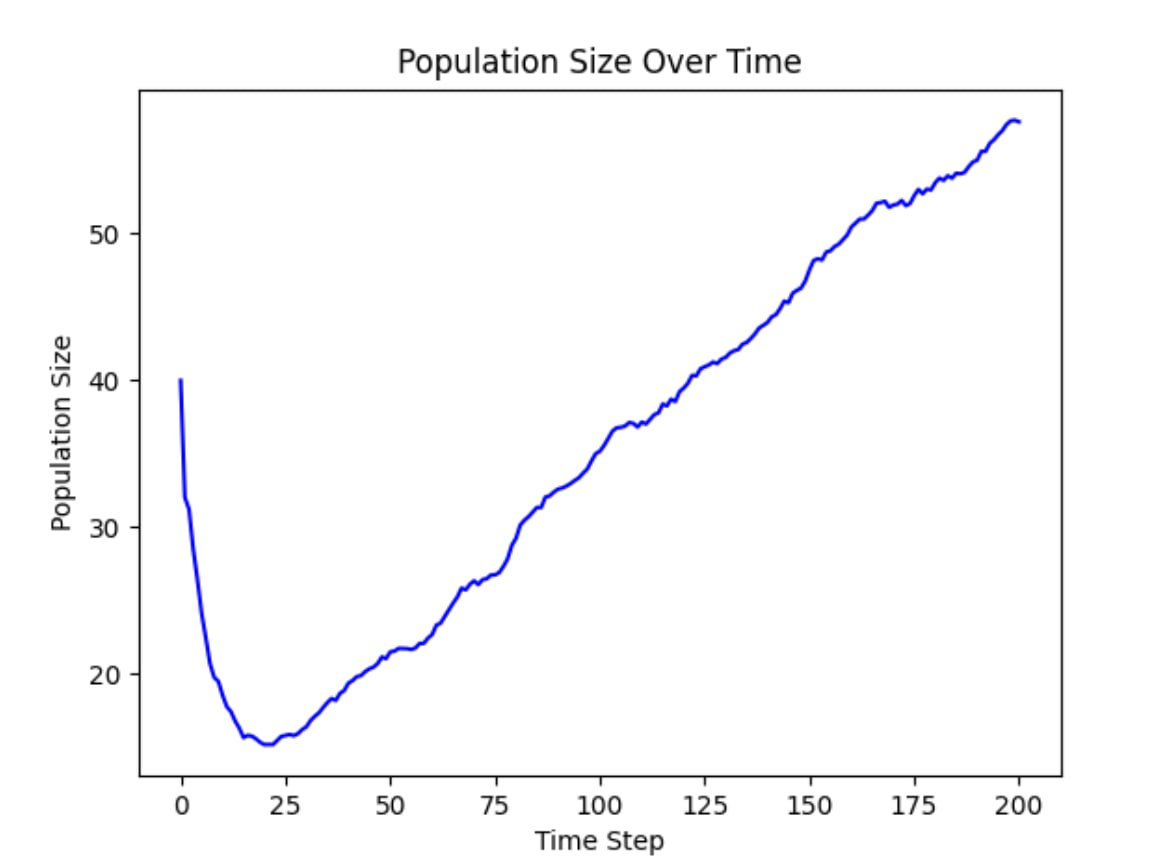
\includegraphics[scale=0.2]{images/image1.jpg}
\end{center}
\begin{center}
    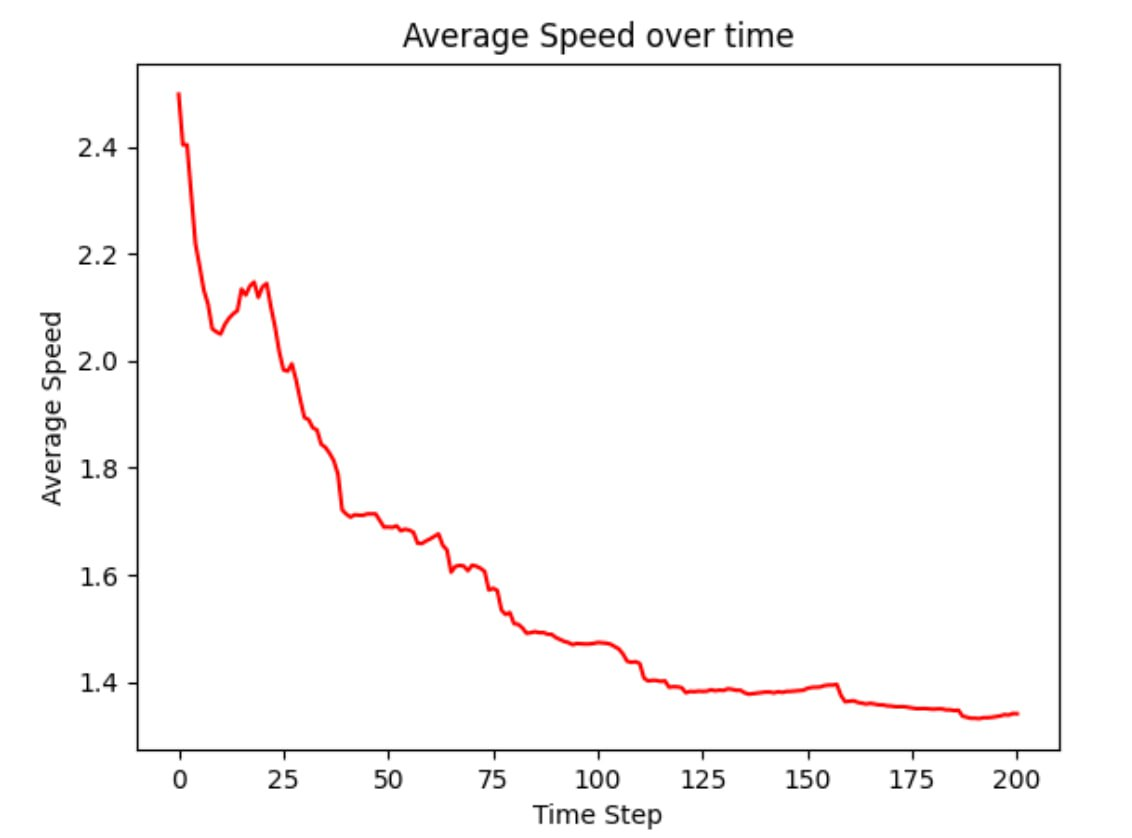
\includegraphics[scale=0.2]{images/image2.jpg}
\end{center}
Code is availabe at \href{https://github.com/suren2003ah7/EvolutionaryModel}{https://github.com/suren2003ah7/EvolutionaryModel}.
\section{Discussion}
We have simulated the model with several cases, however we may try on more complex cases.

\begin{enumerate}
    \item Random genes. Try many random genes for creatures and see if we reach equilibrium of one gene.
    \item Strong specific genes. Start with high values for specific genes and see if we reach equilibrium or not after mutaitons.
    \item Record the evolution of each gene by averaging that genes during each timestep.
\end{enumerate}
\nocite{*}
\bibliographystyle{apacite}
\bibliography{refs}
\end{document}